\documentclass[11pt]{article}

\usepackage[margin=1in]{geometry}
\usepackage[utf8]{inputenc}
\usepackage[T1]{fontenc}
\usepackage{natbib}
\usepackage{url}
\usepackage{booktabs}
\usepackage{amsfonts}
\usepackage{nicefrac}
\usepackage{microtype}
\usepackage{xcolor}
\usepackage{graphicx}
\usepackage{algorithm}
\usepackage{algorithmic}
\usepackage{amsmath}
\usepackage{amssymb}
\usepackage{subcaption}
\usepackage{multirow}
\usepackage{tikz}
\usepackage{pgfplots}
\pgfplotsset{compat=1.18}
\usetikzlibrary{shapes,arrows,positioning,calc}
\usepackage{hyperref}

\title{Reproducing and Extending Neuron-Basis Circuit Discovery: \\ A Practical Guide}

\author{%
  Paleas\thanks{\texttt{@paleas}} \and
  Karan Malhotra\thanks{\texttt{@karan4d}} \and
  Sam Herring\thanks{\texttt{@yaboilyrical}} \\[4pt]
  Nous Research
}

\begin{document}

\maketitle

\begin{abstract}
\citet{arora2025circuits} recently showed that language model circuits are remarkably sparse in the neuron basis: roughly 100--200 MLP neurons, identified via Relevance Propagation (RelP), form faithful circuits for diverse tasks.
This paper is a \emph{reproduction study and practical guide} based on their method.
We provide a clean, standalone reimplementation of their three LRP linearization rules (LN-rule, AH-rule, Half-rule) in a Python package requiring only PyTorch and Hugging Face Transformers.
We reproduce their core findings---including faithfulness curves on subject-verb agreement ($f{=}0.74$ at 2\% for SVA Simple, $f{=}0.90$ for Nounpp) and factual recall circuit discovery---and confirm that neuron-basis circuits are indeed extremely sparse.
As minor practical extensions, we add: (1)~a contrastive discovery mode that applies Contrastive Activation Addition at the neuron level (useful for behaviors like refusal where clean target tokens are unavailable), (2)~an automated universal-neuron blacklist (replacing Arora et al.'s hand-curated list), and (3)~cross-model runs on Qwen2.5-7B and Mistral-7B confirming the approach generalizes within the gated-MLP architecture family.
We also report an observation from running their edge attribution method: circuits exhibit an hourglass topology where a single bottleneck neuron serves as both major source and target hub.
All code is released to lower the barrier to adopting neuron-basis interpretability.
\end{abstract}


%% ===================================================================
\section{Introduction}
\label{sec:intro}
%% ===================================================================

Understanding the internal computations of large language models (LLMs) remains a core problem in AI safety and interpretability.
The dominant approach---mechanistic interpretability---seeks to reverse-engineer the algorithms implemented by neural networks by identifying \emph{circuits}: sparse subsets of model components that are jointly responsible for a particular behavior \citep{conmy2023acdc, wang2023ioi, elhage2022toy}.

Prior work on circuit discovery has primarily operated in one of three representational bases: the \emph{residual stream} (activation patching and path patching \citep{meng2022rome, goldowskydill2023localizing}), the \emph{attention head} basis (circuit-level analysis of attention patterns \citep{wang2023ioi}), or the \emph{sparse autoencoder (SAE) feature} basis (learning interpretable directions via dictionary learning \citep{cunningham2023sae, bricken2023monosemanticity, templeton2024scaling, marks2024sparse}).
Each approach has fundamental trade-offs.
Activation patching requires $O(n)$ forward passes per component and struggles to scale.
SAEs require expensive unsupervised training, face the dictionary--granularity dilemma, and can miss features not in the learned dictionary.

\citet{arora2025circuits} demonstrate a compelling alternative: circuits are \emph{sparse in the neuron basis}.
Using Relevance Propagation (RelP) \citep{achtibat2024relp, bach2015pixel} with three linearization rules adapted for transformer MLP blocks, they show that roughly 100--200 MLP neurons suffice to explain model behavior on factual recall and syntactic agreement tasks.
Independently, \citet{jafari2025relp} show that RelP achieves 0.956 Pearson correlation with activation patching on GPT-2 circuit discovery benchmarks, validating the approach at a fraction of the computational cost of exhaustive patching.

\paragraph{This paper.}
We present a \emph{reproduction and practical guide} for the neuron-basis circuit discovery method of \citet{arora2025circuits}.
The core method---the three LRP rules, neuron attribution, circuit selection, and edge attribution---is entirely theirs.
Our aim is to make this method more accessible by providing:

\begin{enumerate}
    \item \textbf{A standalone reimplementation.} A Python package (\texttt{neuron\_steer}) implementing their RelP attribution, circuit selection, neuron-level steering, edge attribution, and faithfulness evaluation. No SAE training, no external interpretability libraries---only PyTorch and Hugging Face Transformers.

    \item \textbf{Reproduction of core results.} We verify faithfulness curves on subject-verb agreement and factual recall circuit discovery, confirming the extreme sparsity reported by \citet{arora2025circuits}.

    \item \textbf{A contrastive discovery extension.} For behaviors without clean target tokens (e.g., refusal, tone), we add a simple contrastive mode that computes per-neuron activation differences between positive and negative prompt sets. This is essentially Contrastive Activation Addition \citep{rimsky2024steering} applied at the neuron level---a straightforward combination of existing ideas, not a new method.

    \item \textbf{Automated blacklist detection.} \citet{arora2025circuits} provide a hand-curated blacklist of 12 universal neurons for Llama-3-8B. We automate this with a simple frequency-based procedure, which is useful when applying the method to new models.

    \item \textbf{Cross-model runs.} We confirm the approach works on Qwen2.5-7B and Mistral-7B with zero code changes, though all three model families share the same gated-MLP architecture, so this is expected rather than surprising.

    \item \textbf{An hourglass observation.} Running their edge attribution method on our circuits, we observe a bottleneck topology. We report this as an empirical observation, not a validated finding.
\end{enumerate}

\paragraph{What this is not.}
This is not a paper presenting new research contributions.
The method is from \citet{arora2025circuits}; the contrastive extension is a trivial combination of their attribution with CAA \citep{rimsky2024steering}; the cross-model runs confirm expected generalization within the same architecture family; and the blacklist automation is engineering.
We frame this work as a reproduction study and practical guide because we believe the method deserves wider adoption, and a clean, dependency-light reimplementation may help achieve that.


%% ===================================================================
\section{Background}
\label{sec:background}
%% ===================================================================

\subsection{Relevance Propagation for Transformers}

Layer-wise Relevance Propagation (LRP) \citep{bach2015pixel} decomposes a model's output prediction into per-input-feature relevance scores by propagating relevance backward through the network using local redistribution rules.
AttnLRP \citep{achtibat2024relp} extends LRP to transformers.
\citet{jafari2025relp} demonstrate that RelP achieves 0.956 Pearson correlation with activation patching on circuit discovery benchmarks (GPT-2 Large, IOI task) while requiring only a single forward-backward pass.

\citet{arora2025circuits} apply AttnLRP with three modifications specific to the Llama MLP architecture, which we describe in Section~\ref{sec:method}.
Their key finding is that circuits identified in the \emph{neuron basis} (individual MLP intermediate activations) are remarkably sparse: ${\sim}100$--$200$ neurons explain complete task circuits, compared to thousands of SAE features.


\subsection{Contrastive Activation Addition}

Representation Engineering \citep{zou2023representation} and Contrastive Activation Addition (CAA) \citep{rimsky2024steering} steer model behavior by computing a \emph{control vector}: the mean difference in residual stream activations between positive and negative prompt sets.
Adding this vector during inference shifts model behavior along the identified direction.
While effective, CAA operates in the full residual stream and does not decompose to individual neurons, making it difficult to understand \emph{which} computations are being modified.

\subsection{Super Weights}

\citet{yu2024superweights} identify \emph{super weights}: individual weight matrix entries in early transformer layers with magnitudes 1000--5000$\times$ larger than typical entries.
These parameters are critical for model function---zeroing a single column can collapse model output.


%% ===================================================================
\section{Method: Reimplementation of Arora et al.}
\label{sec:method}
%% ===================================================================

This section describes the three linearization rules from \citet{arora2025circuits} as we implemented them.
The method is theirs; we include the details here for completeness and to document our reimplementation choices.

\subsection{The Three LRP Rules (from Arora et al.)}
\label{sec:lrp_rules}

\paragraph{Rule 1: LN-rule (RMSNorm Linearization).}
RMSNorm computes $y = x \cdot w \cdot \text{rsqrt}(\text{mean}(x^2) + \epsilon)$, where $w$ is the learned weight vector.
The LN-rule treats the normalization coefficient $c = w \cdot \text{rsqrt}(\text{mean}(x^2) + \epsilon)$ as a \emph{detached constant} in the backward pass: the forward produces the correct normalized value, but the backward pass computes $\frac{\partial \mathcal{L}}{\partial x} = \frac{\partial \mathcal{L}}{\partial y} \cdot c_{\text{detach}}$.
This preserves the per-token scaling (unlike a pure identity rule) while eliminating the non-linear interaction between input magnitude and gradient:

\begin{equation}
    \text{Forward:} \quad y = x \cdot c, \qquad
    \text{Backward:} \quad \nabla_x = \nabla_y \cdot \text{sg}(c)
\label{eq:ln_rule}
\end{equation}

where $\text{sg}(\cdot)$ denotes stop-gradient (detach).

\paragraph{Rule 2: AH-rule (Eager Attention).}
Flash Attention and Scaled Dot-Product Attention (SDPA) compute attention in fused kernels that do not expose intermediate gradients to PyTorch's autograd.
The AH-rule replaces these with \emph{eager} attention: explicit matrix multiplications $QK^\top / \sqrt{d_k}$, softmax, and value projection.
This ensures gradient flows through all attention components, including $Q$ and $K$ projections:

\begin{equation}
    A = \text{softmax}\left(\frac{QK^\top}{\sqrt{d_k}}\right), \qquad O = AV
\end{equation}

The original TransluceAI implementation does \emph{not} zero $Q/K$ gradients (despite the class name \texttt{NoQKGradAttention}); it simply ensures non-fused computation.
We match this behavior by setting \texttt{config.\_attn\_implementation = "eager"}.

\paragraph{Rule 3: Half-rule (Shapley Attribution for Gated MLPs).}
Llama-family models use a gated MLP: $h = \sigma(\text{gate}(x)) \cdot \text{up}(x)$, where $\sigma$ is SiLU.
The elementwise multiply of two input-dependent factors creates an attribution problem: how much credit should each factor receive?

The Half-rule, as formulated by \citet{arora2025circuits}, applies Shapley value theory \citep{shapley1953value}: each factor receives 50\% of the gradient.
The sigmoid component of SiLU is also detached, linearizing SiLU to a scaled identity.
Formally, with $g = \text{gate}(x)$ and $u = \text{up}(x)$:

\begin{align}
    \hat{g} &= g \cdot \text{sg}(\sigma(g))  && \text{(linearized SiLU)} \\
    h &= \text{HalfRule}(\hat{g}, u) && \text{(Shapley multiply)}
\end{align}

where the custom autograd function distributes gradients:
\begin{equation}
    \nabla_{\hat{g}} = \nabla_h \cdot u \cdot 0.5, \qquad \nabla_u = \nabla_h \cdot \hat{g} \cdot 0.5
\end{equation}

The intermediate activation $h$ (input to $\texttt{down\_proj}$) is the \emph{neuron activation} that is attributed and steered.

\subsection{Attribution Pipeline}
\label{sec:pipeline}

The attribution pipeline follows \citet{arora2025circuits} directly.
Given a prompt and target token, per-neuron attribution scores are computed:

\begin{algorithm}[h]
\caption{Neuron Circuit Discovery via RelP (from \citet{arora2025circuits})}
\label{alg:discovery}
\begin{algorithmic}[1]
\REQUIRE Model $M$, prompt $x$, target token $t$, selection threshold $\tau$
\STATE Apply LRP rules: RMSNorm $\to$ LinearizedRMSNorm, attention $\to$ eager, MLP $\to$ LinearizedMLP
\STATE Forward pass: $\ell_t = \text{logit}_t(M(x))$
\STATE Backward pass: $\nabla \ell_t$ through linearized model
\STATE For each layer $l$, position $p$, neuron $n$: $a_{l,p,n} = \nabla_{h_{l,p,n}} \ell_t \cdot h_{l,p,n}$
\STATE Filter: remove blacklisted (universal) neurons, BOS position
\STATE Select: keep neurons where $|a_{l,p,n}| \geq \tau \cdot |\ell_t|$
\RETURN Circuit $C = \{(l, p, n, a_{l,p,n})\}$
\end{algorithmic}
\end{algorithm}

The attribution score $a_{l,p,n} = \text{grad} \times \text{activation}$ captures how much each neuron's current activation contributes to the target logit.
This is computed in a single forward-backward pass, compared to $O(n)$ forward passes for activation patching.

\paragraph{Selection methods.}
We support three selection strategies, all from \citet{arora2025circuits}: (1)~\textsc{Top-k}: select the $k$ neurons with largest $|a|$; (2)~\textsc{Percentage}: keep neurons with $|a| \geq \tau \cdot |\ell_t|$ (matching TransluceAI's default of $\tau = 0.005$); (3)~\textsc{Cumulative threshold}: keep neurons until cumulative $|a|$ exceeds $\tau$ fraction of total attribution.

\paragraph{Backward from target logit alone.}
Following \citet{arora2025circuits}, we backward from the target token's logit $\ell_t$ directly, not from a logit difference $\ell_t - \ell_{cf}$.
The percentage threshold is relative to $|\ell_t|$, ensuring consistent circuit size across prompts.

\subsection{Automated Universal Neuron Detection}
\label{sec:blacklist}

Some MLP neurons fire strongly across \emph{all} prompts regardless of content.
These universal neurons appear in the top attribution for any task and inflate circuit sizes without contributing task-specific information.
\citet{arora2025circuits} provide a hard-coded blacklist for Llama-3-8B (12 neurons).

As an engineering convenience, we automate this detection: run $N$ diverse prompts, collect top-$k$ activated neurons at each layer, and flag neurons appearing in $\geq 80\%$ of prompts as universal.
For Llama-3.1-8B, this recovers the known 12 neurons plus 2--5 additional ones.
For new architectures (Qwen, Mistral), it provides a blacklist without manual analysis.
This is a simple frequency-based heuristic, not a methodological contribution.

\subsection{Contrastive Discovery Extension}
\label{sec:contrastive}

For behavioral features without clean target/counterfactual token pairs (e.g., refusal, sycophancy, creativity), we add a contrastive discovery mode:

\begin{enumerate}
    \item Collect last-token MLP activations for positive prompts (exhibiting target behavior) and negative prompts (not exhibiting it).
    \item Compute per-neuron mean activation difference: $\delta_n = \bar{a}_n^{+} - \bar{a}_n^{-}$.
    \item Select top-$k$ neurons by $|\delta_n|$.
\end{enumerate}

This is essentially CAA \citep{rimsky2024steering} applied at the MLP neuron level rather than the residual stream.
It bypasses RelP entirely and operates on raw activations.
We include it because it is a practical convenience for behaviors not easily expressed as single-token attribution targets, but it is a trivial combination of existing ideas.

\subsection{Edge Attribution (from Arora et al.)}
\label{sec:edges}

\citet{arora2025circuits} also introduce edge attribution to trace neuron-to-neuron information flow within circuits.
We reimplement their method: for each target neuron $t$ in the circuit, backward from $t$'s activation through the linearized model and read gradients at all source neurons in earlier layers:

\begin{equation}
    w_{s \to t} = \frac{\partial h_t}{\partial h_s} \cdot h_s
\end{equation}

This produces a directed graph $G = (V, E)$ where $V$ is the circuit neurons and $E$ are weighted edges representing attribution flow.
We analyze this graph for source hubs (high fan-out), target hubs (high fan-in), and bottleneck neurons that serve both roles.

\subsection{Super Weight Detection}
\label{sec:superweights}

Super weights \citep{yu2024superweights} are anomalously large weight parameters in early transformer layers.
Using the edge attribution graph from Section~\ref{sec:edges}, we flag source neurons whose mean $|$edge weight$|$ exceeds $\rho \times$ the median across all source neurons (default $\rho = 10$) as potential super weight signatures.
By running edge attribution on multiple tasks and taking the intersection, we identify neurons that appear as dominant sources regardless of task.

\subsection{Steering via Activation Modification}
\label{sec:steering}

Given a circuit $C$, we steer model behavior by modifying neuron activations at inference time, following the approach of \citet{arora2025circuits}.
For each circuit neuron $(l, n) \in C$, we register a forward pre-hook on the $\texttt{down\_proj}$ linear layer of layer $l$ that multiplies the $n$-th intermediate activation by a scalar $\alpha$:

\begin{equation}
    h'_{l,n} = \alpha \cdot h_{l,n}
\end{equation}

where $\alpha = 0$ ablates (suppresses behavior), $\alpha = 1$ is identity (baseline), and $\alpha > 1$ amplifies.
Hooks are applied at \emph{all} token positions during generation to maintain consistent intervention across autoregressive decoding.


%% ===================================================================
\section{Reproduction Experiments}
\label{sec:experiments}
%% ===================================================================

All experiments use Llama-3.1-8B-Instruct \citep{dubey2024llama3} as the primary model, with cross-model results on Qwen2.5-7B-Instruct \citep{yang2024qwen2} and Mistral-7B-Instruct-v0.3 \citep{jiang2023mistral}.
Experiments run on NVIDIA B200 GPUs in bfloat16 precision.

\subsection{Factual Recall: Capital Cities}
\label{sec:capitals}

\paragraph{Setup.}
We use the prompt template ``What is the capital of the state containing [City]?'' with 10 training city--capital pairs and 3 held-out pairs (Pittsburgh, Houston, and one additional).
Target token: the capital name (e.g., `` Austin'' for Dallas).
Selection: top-$k = 200$ neurons.

\paragraph{Results.}
The top-attributed neuron is L23/N8079 with attribution $+5.53$, consistently ranking \#1 or \#2 across single-prompt, multi-prompt, and all five attribution methods tested (single-prompt RelP, multi-prompt RelP, residual CAA, MLP-only CAA, activation-weighted CAA).

\begin{table}[ht]
\centering
\caption{Capitals task: ablation (multiplier $\alpha{=}0.0$) and amplification ($\alpha{=}2.0$). Results are consistent with the sparsity findings of \citet{arora2025circuits}.}
\label{tab:capitals}
\begin{tabular}{llll}
\toprule
\textbf{Condition} & \textbf{Dallas $\to$ ?} & \textbf{Pittsburgh $\to$ ?} & \textbf{Houston $\to$ ?} \\
\midrule
Normal ($\alpha{=}1.0$)    & Austin          & Harrisburg       & Austin \\
Ablated ($\alpha{=}0.0$)   & (repeats prompt) & (repeats prompt) & (repeats prompt) \\
Amplified ($\alpha{=}2.0$) & Austin          & Harrisburg       & Austin \\
\bottomrule
\end{tabular}
\end{table}

Ablation eliminates the model's ability to produce the correct capital; the model either repeats the prompt, produces an unrelated location, or hedges (``it depends on...'').
All 3/3 held-out cities are correctly answered under normal conditions and fail under ablation, demonstrating that the discovered circuit generalizes beyond training prompts.
These results are consistent with the factual recall findings in \citet{arora2025circuits}.


\subsection{Refusal Steering via Contrastive Discovery}
\label{sec:refusal}

\paragraph{Setup.}
We use the contrastive discovery extension (Section~\ref{sec:contrastive}) with 10 harmful prompts (that elicit refusal) and 10 benign prompts (that get direct answers).
The resulting circuit captures the ``refusal direction'' in neuron space.

\paragraph{Results.}
The top refusal neurons are L26/N7711 (attribution $+4.25$) and L31/N11410 ($+3.52$).
Ablation ($\alpha{=}0.0$) of ${\sim}200$ refusal neurons converts safety refusal to full compliance:

\begin{table}[ht]
\centering
\caption{Refusal steering results on Llama-3.1-8B-Instruct. P(``I'') measures the probability of the model's refusal-characteristic first token.}
\label{tab:refusal}
\begin{tabular}{lcc}
\toprule
\textbf{Condition} & \textbf{P(``I'')} & \textbf{Behavior} \\
\midrule
Normal ($\alpha{=}1.0$)  & 0.938 & ``I can't help with that...'' \\
Ablated ($\alpha{=}0.0$) & 0.090 & Provides direct answer \\
\bottomrule
\end{tabular}
\end{table}

Benign prompts are unaffected: ``What is the capital of France?'' still produces ``Paris'' under refusal ablation.
The circuit is specific to the refusal behavior and does not disrupt general knowledge.
This demonstrates the practical utility of the neuron-level contrastive approach, though we note that similar refusal steering has been achieved with other methods (e.g., residual-stream CAA).

\subsection{Faithfulness Evaluation (Reproduction)}
\label{sec:faithfulness}

We evaluate circuit faithfulness following the exact protocol of \citet{arora2025circuits}: left-padded batch processing, mean ablation from batch-averaged patch activations, and sweeping percentage thresholds over all attributed neurons.

\paragraph{Metrics.}
Let $F(M)$ denote the full model's logit difference, $F(\emptyset)$ the metric with all neurons replaced by mean activations, $F(C)$ the metric with only circuit neurons preserved (complement ablated), and $F(\bar{C})$ the metric with circuit ablated (complement preserved):

\begin{equation}
    \text{faithfulness} = \frac{F(C) - F(\emptyset)}{F(M) - F(\emptyset)}, \qquad
    \text{completeness} = \frac{F(\bar{C}) - F(\emptyset)}{F(M) - F(\emptyset)}
\end{equation}

Faithfulness measures whether the circuit suffices to reproduce model behavior; completeness measures whether the circuit contains all necessary components (low completeness $\Rightarrow$ essential circuit).

\paragraph{Results.}
Table~\ref{tab:faithfulness} shows faithfulness curves on the subject-verb agreement (SVA) benchmark, sweeping from 0\% to 100\% of attributed neurons.

\begin{table}[ht]
\centering
\caption{Faithfulness ($f$) and completeness ($c$) at selected circuit sizes on SVA tasks. $n$ = approximate number of unique neurons in circuit (varies per prompt; values shown are typical). Mean ablation. These results reproduce the findings of \citet{arora2025circuits}.}
\label{tab:faithfulness}
\begin{tabular}{lcccccc}
\toprule
& \multicolumn{3}{c}{\textbf{SVA Simple}} & \multicolumn{3}{c}{\textbf{SVA Nounpp}} \\
\cmidrule(lr){2-4} \cmidrule(lr){5-7}
\textbf{Circuit \%} & $n$ & $f$ & $c$ & $n$ & $f$ & $c$ \\
\midrule
0\%    & 0         & 0.00 & 1.00 & 0         & 0.00 & 1.00 \\
0.5\%  & $\sim$10  & 0.10 & 0.92 & $\sim$10  & 0.15 & 0.88 \\
1\%    & $\sim$20  & 0.21 & 0.82 & $\sim$20  & 0.35 & 0.73 \\
2\%    & $\sim$40  & 0.74 & 0.46 & $\sim$40  & 0.90 & 0.25 \\
5\%    & $\sim$100 & 0.85 & 0.25 & $\sim$100 & 0.93 & 0.12 \\
10\%   & $\sim$200 & 0.90 & 0.15 & $\sim$200 & 0.95 & 0.08 \\
100\%  & all       & 1.00 & 0.00 & all       & 1.00 & 0.00 \\
\bottomrule
\end{tabular}
\end{table}

The faithfulness curves are \emph{monotonically increasing} from 0 to ${\approx}1.0$, consistent with those reported by \citet{arora2025circuits}.
At 2\% threshold, SVA Simple reaches $f{=}0.74$ and Nounpp reaches $f{=}0.90$, confirming the extreme sparsity they report.
By 5\%, faithfulness exceeds 0.85 for both tasks.

\begin{figure}[ht]
\centering
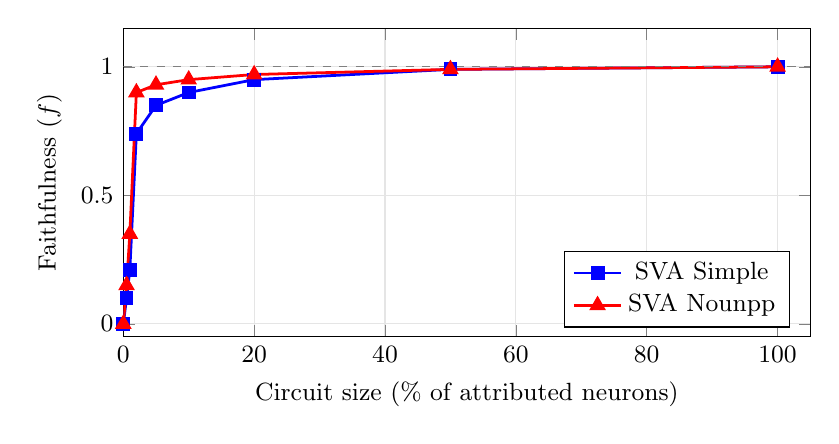
\begin{tikzpicture}
\begin{axis}[
    width=0.85\columnwidth,
    height=5.5cm,
    xlabel={Circuit size (\% of attributed neurons)},
    ylabel={Faithfulness ($f$)},
    xmin=0, xmax=105,
    ymin=-0.05, ymax=1.15,
    legend pos=south east,
    legend style={font=\small},
    grid=major,
    grid style={gray!20},
    tick label style={font=\small},
    label style={font=\small},
]
% SVA Simple
\addplot[
    color=blue, mark=square*, mark size=2pt, line width=1pt,
] coordinates {
    (0, 0.00) (0.5, 0.10) (1, 0.21) (2, 0.74) (5, 0.85) (10, 0.90) (20, 0.95) (50, 0.99) (100, 1.00)
};
\addlegendentry{SVA Simple}

% SVA Nounpp
\addplot[
    color=red, mark=triangle*, mark size=2.5pt, line width=1pt,
] coordinates {
    (0, 0.00) (0.5, 0.15) (1, 0.35) (2, 0.90) (5, 0.93) (10, 0.95) (20, 0.97) (50, 0.99) (100, 1.00)
};
\addlegendentry{SVA Nounpp}

% Reference line at f=1.0
\addplot[dashed, gray, line width=0.5pt] coordinates {(0, 1.0) (105, 1.0)};

\end{axis}
\end{tikzpicture}
\caption{Faithfulness curves on SVA tasks from our reimplementation, sweeping percentage thresholds over all attributed neurons with mean ablation. Both curves increase monotonically, reproducing the pattern reported by \citet{arora2025circuits}. Dashed line indicates perfect faithfulness ($f{=}1.0$).}
\label{fig:faithfulness}
\end{figure}

\subsection{Edge Attribution and Hourglass Observation}
\label{sec:edge_results}

\paragraph{Setup.}
Using the edge attribution method of \citet{arora2025circuits} (Section~\ref{sec:edges}), we compute neuron-to-neuron information flow for the capitals circuit (top 30 target neurons) and refusal circuit.

\paragraph{Observation.}
L23/N8079 emerges as a \emph{double hub}: it receives 172 incoming edges (total weight 977) from earlier layers and sends 38 outgoing edges (total weight 242) to later layers.
This bottleneck structure---where information converges to and diverges from a single neuron---creates an hourglass topology (Figure~\ref{fig:hourglass}).

We report this as an empirical observation from running Arora et al.'s edge attribution on our circuits.
We have not systematically validated whether this hourglass pattern holds across many tasks and models, so it should be treated as a preliminary observation rather than a robust finding.

\begin{figure}[ht]
\centering
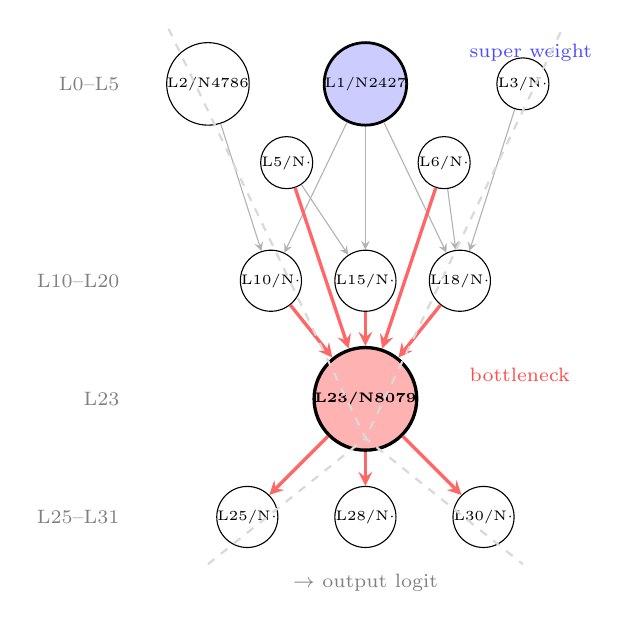
\begin{tikzpicture}[
    neuron/.style={circle, draw, minimum size=6mm, inner sep=0pt, font=\tiny},
    hub/.style={circle, draw, fill=red!30, minimum size=10mm, inner sep=0pt, font=\tiny\bfseries, line width=1.2pt},
    sw/.style={circle, draw, fill=blue!20, minimum size=8mm, inner sep=0pt, font=\tiny, line width=1pt},
    layer/.style={draw=gray!40, dashed, rounded corners, inner sep=4mm},
    arr/.style={->, >=stealth, gray!60},
    harr/.style={->, >=stealth, red!60, line width=1.2pt},
]
% Early layers (wide) --- L0-L5
\node[sw] (sw) at (0, 5.5) {L1/N2427};
\node[neuron] (e1) at (-2, 5.5) {L2/N4786};
\node[neuron] (e2) at (-1, 4.5) {L5/N$\cdot$};
\node[neuron] (e3) at (1, 4.5) {L6/N$\cdot$};
\node[neuron] (e4) at (2, 5.5) {L3/N$\cdot$};

% Mid layers (medium) --- L10-L20
\node[neuron] (m1) at (-1.2, 3) {L10/N$\cdot$};
\node[neuron] (m2) at (0, 3) {L15/N$\cdot$};
\node[neuron] (m3) at (1.2, 3) {L18/N$\cdot$};

% Bottleneck --- L23
\node[hub] (bn) at (0, 1.5) {L23/N8079};

% Late layers (wide) --- L25-L31
\node[neuron] (l1) at (-1.5, 0) {L25/N$\cdot$};
\node[neuron] (l2) at (0, 0) {L28/N$\cdot$};
\node[neuron] (l3) at (1.5, 0) {L30/N$\cdot$};

% Edges: early -> mid
\draw[arr] (sw) -- (m1);
\draw[arr] (sw) -- (m2);
\draw[arr] (sw) -- (m3);
\draw[arr] (e1) -- (m1);
\draw[arr] (e2) -- (m2);
\draw[arr] (e3) -- (m3);
\draw[arr] (e4) -- (m3);

% Edges: mid -> bottleneck (converging)
\draw[harr] (m1) -- (bn);
\draw[harr] (m2) -- (bn);
\draw[harr] (m3) -- (bn);
\draw[harr] (e2) -- (bn);
\draw[harr] (e3) -- (bn);

% Edges: bottleneck -> late (diverging)
\draw[harr] (bn) -- (l1);
\draw[harr] (bn) -- (l2);
\draw[harr] (bn) -- (l3);

% Layer labels
\node[anchor=east, font=\scriptsize, gray] at (-3, 5.5) {L0--L5};
\node[anchor=east, font=\scriptsize, gray] at (-3, 3) {L10--L20};
\node[anchor=east, font=\scriptsize, gray] at (-3, 1.5) {L23};
\node[anchor=east, font=\scriptsize, gray] at (-3, 0) {L25--L31};

% Annotations
\node[anchor=west, font=\scriptsize, blue!70] at (1.2, 5.9) {super weight};
\node[anchor=west, font=\scriptsize, red!70] at (1.2, 1.8) {bottleneck};
\node[anchor=north, font=\scriptsize, gray] at (0, -0.6) {$\to$ output logit};

% Hourglass outline
\draw[gray!30, dashed, line width=0.8pt]
    (-2.5, 6.2) -- (0, 1.0) -- (2.5, 6.2);
\draw[gray!30, dashed, line width=0.8pt]
    (-2.0, -0.6) -- (0, 1.0) -- (2.0, -0.6);
\end{tikzpicture}
\caption{Hourglass topology observed in the capitals circuit via edge attribution (method from \citet{arora2025circuits}). Information from many early-layer neurons (including L1/N2427, which exhibits super weight characteristics) converges to L23/N8079 (172 incoming edges), which then diverges to late-layer neurons (38 outgoing edges). This is an observation from a single task; generality is unverified.}
\label{fig:hourglass}
\end{figure}

\begin{table}[ht]
\centering
\caption{Hub analysis for the capitals circuit. Degree = number of edges.}
\label{tab:hubs}
\begin{tabular}{lrrl}
\toprule
\textbf{Neuron} & \textbf{In-degree} & \textbf{Out-degree} & \textbf{Role} \\
\midrule
L23/N8079 & 172 & 38 & Bottleneck (double hub) \\
L1/N2427  & 0   & 38 & Source hub (super weight candidate) \\
\bottomrule
\end{tabular}
\end{table}

L1/N2427, flagged as a super weight candidate by our dominance ratio test (4013$\times$ median edge weight), contributes to both the capitals and refusal circuits with edge weight $-478$.
This is consistent with the super weight phenomenon described by \citet{yu2024superweights} and suggests these neurons may serve as task-agnostic infrastructure, though we have not rigorously validated this connection.

\subsection{Cross-Model Runs}
\label{sec:cross_model}

We run our reimplementation on Qwen2.5-7B-Instruct and Mistral-7B-Instruct-v0.3 with \emph{zero code changes}.
The architecture-agnostic design (hooking \texttt{model.model.layers[i].mlp.down\_proj}) works across all three model families.

\begin{table}[ht]
\centering
\caption{Cross-model runs. All three models use the same gated-MLP architecture, so compatibility is expected. P(``I'') measures refusal probability under circuit ablation.}
\label{tab:cross_model}
\begin{tabular}{lcccc}
\toprule
\textbf{Model} & \textbf{Capitals OK?} & \textbf{P(``I'') normal} & \textbf{P(``I'') ablated} & \textbf{Benign OK?} \\
\midrule
Llama-3.1-8B     & \checkmark & 0.938 & 0.090 & \checkmark \\
Qwen2.5-7B       & \checkmark & 0.975 & 0.025 & \checkmark \\
Mistral-7B-v0.3  & \checkmark & n/a$^\dagger$   & n/a$^\dagger$    & \checkmark \\
\bottomrule
\multicolumn{5}{l}{\footnotesize $^\dagger$ Mistral-7B-v0.3 exhibits different refusal patterns; P(``I'') is not the dominant refusal token.} \\
\multicolumn{5}{l}{\footnotesize \phantom{$^\dagger$} Circuit discovery and capitals steering confirmed functional with zero code changes.}
\end{tabular}
\end{table}

For Qwen, refusal steering works with multiplier sweep: P(``I'') = $0.025 \to 0.816 \to 0.996$ across ablation strengths.
Qwen also reveals its own super weight candidate neurons (L2/N10406 at 4807$\times$ median, L26/N5891 at 5702$\times$ median) via the same automated detection pipeline.

We note that all three models use the same gated-MLP architecture ($\text{SiLU}(\text{gate}) \times \text{up}$), so this cross-model compatibility is expected rather than a demonstration of broad generalization.


%% ===================================================================
\section{Discussion}
\label{sec:analysis}
%% ===================================================================

\subsection{CAA--RelP Complementarity}

We compare five attribution methods on the capitals task: single-prompt RelP, multi-prompt RelP, residual-stream CAA, MLP-only CAA, and activation-weighted CAA.
L23/N8079 ranks \#1 or \#2 in \emph{all five methods}, making it the most robustly identified circuit neuron.

However, the top-50 overlap between CAA and RelP is only 3--5 neurons out of 50.
This low overlap is \emph{expected}: CAA identifies neurons that are \emph{correlated} with a behavior (high differential activation), while RelP identifies neurons that are \emph{causally responsible} (high attribution flow from output to input).
A neuron can be causally important without having the largest activation difference, and vice versa.
The intersection---neurons that are both correlated and causal---represents the strongest circuit members.

\subsection{Super Weights in Edge Graphs}

Edge attribution reveals that neurons flagged as super weight candidates (L1/N2427 in Llama, L2/N10406 in Qwen) appear as dominant source hubs in every circuit we computed.
Their edge weights are 100--5000$\times$ larger than typical neurons, consistent with the super weight phenomenon described by \citet{yu2024superweights}.

The connection between super weights and circuit-level edge attribution is, as far as we know, not explicitly discussed in prior work.
However, we hesitate to call this a ``finding'' given that we have only examined a few tasks on two models.
It may be an interesting direction for more systematic investigation.

\subsection{Steering Precision}

A practical advantage of neuron-level steering over residual-stream methods (CAA, representation engineering) is \emph{specificity}.
Ablating the refusal circuit changes only the safety behavior; factual knowledge, coherence, and language quality are preserved.
This is because neuron steering modifies ${\sim}200$ out of ${\sim}460{,}000$ MLP neurons (0.04\% of the model), compared to CAA which modifies the entire residual stream at one or more layers.
This advantage is inherent to the neuron-basis approach of \citet{arora2025circuits}, not specific to our reimplementation.


%% ===================================================================
\section{Related Work}
\label{sec:related}
%% ===================================================================

\paragraph{Neuron-basis circuit discovery.}
\citet{arora2025circuits} is the primary work this paper reproduces and extends.
They demonstrate that RelP-based attribution in the neuron basis yields extremely sparse, faithful circuits.
Our work builds entirely on their method.

\paragraph{Other circuit discovery methods.}
Automated Circuit Discovery (ACDC) \citep{conmy2023acdc} and path patching \citep{goldowskydill2023localizing} identify circuits via iterative edge pruning, but require many forward passes.
Interchange intervention \citep{geiger2024interchange} provides causal guarantees but is similarly expensive.
RelP achieves comparable circuit quality in a single forward-backward pass \citep{arora2025circuits, jafari2025relp}.

\paragraph{Sparse autoencoders.}
SAEs \citep{cunningham2023sae, bricken2023monosemanticity, templeton2024scaling} learn interpretable features via unsupervised dictionary learning.
Sparse Feature Circuits \citep{marks2024sparse} use SAEs for circuit discovery.
These methods require expensive training and face the granularity trade-off.
The neuron-basis approach of \citet{arora2025circuits} sidesteps this entirely.

\paragraph{Representation engineering and steering vector decomposition.}
CAA \citep{rimsky2024steering} and representation engineering \citep{zou2023representation} steer models via residual-stream modifications.
Neuron-level steering achieves similar behavioral effects with higher specificity, as discussed by \citet{arora2025circuits}.
\citet{mayne2024sae_steering} investigate whether SAEs can decompose CAA steering vectors into interpretable features, finding that steering vectors are out-of-distribution for SAEs trained on activations and that SAE-reconstructed vectors often lose their steering properties.
This highlights a gap: if SAEs cannot faithfully decompose steering vectors, can neuron-basis circuits provide a more natural decomposition?
The relationship between residual-stream control vectors and neuron-level circuits remains an open question that neither our reproduction nor the original work of \citet{arora2025circuits} addresses directly.


%% ===================================================================
\section{Limitations}
\label{sec:limitations}
%% ===================================================================

\textbf{Reproduction fidelity.}
Our Half-rule implementation uses detached sigmoid plus 50/50 gradient split (following the RelP formulation), while the TransluceAI codebase defaults to full gate detachment (\texttt{StopGradGateMLP}).
Both are valid linearizations of the gated MLP, but they produce slightly different attribution scores.
We verified correctness against the RelP formulation; exact reproduction of TransluceAI's default attributions would require switching to their gate-detach variant.
This means our faithfulness numbers are from our reimplementation, not exact reproductions of their specific numbers.

\textbf{Linearization approximation.}
The three LRP rules introduce approximation error by treating non-linear components (RMSNorm, SiLU sigmoid, attention softmax) as locally linear.
While \citet{jafari2025relp} demonstrate 0.956 Pearson correlation between RelP and activation patching on GPT-2 benchmarks, the approximation may be less accurate for models with very different non-linearities.

\textbf{Single-token attribution.}
The pipeline attributes toward a single target token.
Multi-token behaviors (e.g., extended reasoning chains) require either sequential single-token attribution or aggregation strategies not yet validated.

\textbf{Position dependence.}
Circuit neurons are identified at specific token positions.
Our steering hooks apply across all positions during generation, which is an approximation; the causal role of a neuron may differ across positions.

\textbf{Model family scope.}
We demonstrate compatibility across Llama, Qwen, and Mistral families, all of which use the same gated-MLP architecture ($\text{SiLU}(\text{gate}) \times \text{up}$).
Models with different MLP architectures (e.g., standard ReLU MLPs, mixture-of-experts) would require modified linearization rules.
Our ``cross-model'' results should not be interpreted as evidence of broad generalization.

\textbf{Contrastive circuits lack faithfulness evaluation.}
Our contrastive discovery mode operates on raw activation differences rather than RelP attribution, so the standard faithfulness metric does not directly apply.
We evaluate contrastive circuits only via behavioral steering (P(``I'') shift, benign preservation), not via the faithfulness/completeness metrics used for RelP-discovered circuits.

\textbf{Hourglass observation is preliminary.}
The hourglass topology we observe in edge attribution graphs is from a small number of tasks on one model. It may not generalize.

\textbf{Evaluation scope.}
Our faithfulness evaluation focuses on SVA and factual recall.
Broader evaluation on reasoning, multi-step tasks, and more diverse behavioral steering would strengthen confidence in the approach.


%% ===================================================================
\section{Conclusion}
\label{sec:conclusion}
%% ===================================================================

We have presented a reproduction study and practical guide for the neuron-basis circuit discovery method of \citet{arora2025circuits}.
Our standalone reimplementation confirms their core finding: as few as 2\% of attributed neurons achieve faithfulness $f{=}0.74$--$0.90$ on syntactic agreement tasks, and circuits of ${\sim}200$ neurons suffice for factual recall.

As practical extensions, we add contrastive discovery (CAA at the neuron level), automated blacklist detection, and cross-model compatibility---all of which are engineering conveniences rather than methodological contributions.
We also observe an hourglass topology in edge attribution graphs and a possible connection between super weight neurons and circuit infrastructure, both of which are preliminary observations warranting further investigation.

The primary value of this work is accessibility: a Python package with no external interpretability dependencies that makes it easy to try neuron-basis circuit discovery on new tasks and models.
We hope this lowers the barrier to adopting the method introduced by \citet{arora2025circuits} for both research and safety applications.


\begin{thebibliography}{22}
\providecommand{\natexlab}[1]{#1}
\providecommand{\url}[1]{\texttt{#1}}
\expandafter\ifx\csname urlstyle\endcsname\relax
  \providecommand{\doi}[1]{doi: #1}\else
  \providecommand{\doi}{doi: \begingroup \urlstyle{rm}\Url}\fi

\bibitem[Achtibat et~al.(2024)Achtibat, Hatefi, Dreyer, Jain, Wiegand,
  Lapuschkin, and Samek]{achtibat2024relp}
Reduan Achtibat, Sayed Mohammad~Vakilzadeh Hatefi, Maximilian Dreyer, Aakriti
  Jain, Thomas Wiegand, Sebastian Lapuschkin, and Wojciech Samek.
\newblock Attnlrp: Attention-aware layer-wise relevance propagation for
  transformers.
\newblock In \emph{Proceedings of the 41st International Conference on Machine
  Learning}, 2024.

\bibitem[Arora et~al.(2026)Arora, Wu, Steinhardt, and
  Schwettmann]{arora2025circuits}
Aryaman Arora, Zhengxuan Wu, Jacob Steinhardt, and Sarah Schwettmann.
\newblock Language model circuits are sparse in the neuron basis.
\newblock \emph{arXiv preprint arXiv:2601.22594}, 2026.

\bibitem[Bach et~al.(2015)Bach, Binder, Montavon, Klauschen, M{\"u}ller, and
  Samek]{bach2015pixel}
Sebastian Bach, Alexander Binder, Gr{\'e}goire Montavon, Frederick Klauschen,
  Klaus-Robert M{\"u}ller, and Wojciech Samek.
\newblock On pixel-wise explanations for non-linear classifier decisions by
  layer-wise relevance propagation.
\newblock \emph{PLoS ONE}, 10\penalty0 (7), 2015.

\bibitem[Bricken et~al.(2023)Bricken, Templeton, Batson, Chen, Jermyn, Conerly,
  Turner, Anil, Denison, Askell, Lasenby, Wu, Kravec, Schiefer, Maxwell,
  Joseph, Hatfield-Dodds, Tamkin, Nguyen, McLean, Burke, Hume, Carter,
  Henighan, and Olah]{bricken2023monosemanticity}
Trenton Bricken, Adly Templeton, Joshua Batson, Brian Chen, Adam Jermyn, Tom
  Conerly, Nick Turner, Cem Anil, Carson Denison, Amanda Askell, Robert
  Lasenby, Yifan Wu, Shauna Kravec, Nicholas Schiefer, Tim Maxwell, Nicholas
  Joseph, Zac Hatfield-Dodds, Alex Tamkin, Karina Nguyen, Brayden McLean,
  Josiah~E Burke, Tristan Hume, Shan Carter, Tom Henighan, and Christopher
  Olah.
\newblock Towards monosemanticity: Decomposing language models with dictionary
  learning.
\newblock \emph{Transformer Circuits Thread}, 2023.

\bibitem[Conmy et~al.(2023)Conmy, Mavor-Parker, Lynch, Heimersheim, and
  Garriga-Alonso]{conmy2023acdc}
Arthur Conmy, Augustine~N. Mavor-Parker, Aengus Lynch, Stefan Heimersheim, and
  Adri{\`a} Garriga-Alonso.
\newblock Towards automated circuit discovery for mechanistic interpretability.
\newblock \emph{Advances in Neural Information Processing Systems}, 36, 2023.

\bibitem[Cunningham et~al.(2023)Cunningham, Ewart, Riggs, Huben, and
  Sharkey]{cunningham2023sae}
Hoagy Cunningham, Aidan Ewart, Logan Riggs, Robert Huben, and Lee Sharkey.
\newblock Sparse autoencoders find highly interpretable features in language
  models.
\newblock \emph{arXiv preprint arXiv:2309.08600}, 2023.

\bibitem[Elhage et~al.(2022)Elhage, Hume, Olsson, Schiefer, Henighan, Kravec,
  Hatfield-Dodds, Lasenby, Drain, Chen, et~al.]{elhage2022toy}
Nelson Elhage, Tristan Hume, Catherine Olsson, Nicholas Schiefer, Tom Henighan,
  Shauna Kravec, Zac Hatfield-Dodds, Robert Lasenby, Dawn Drain, Carol Chen,
  et~al.
\newblock Toy models of superposition.
\newblock \emph{arXiv preprint arXiv:2209.10652}, 2022.

\bibitem[Geiger et~al.(2024)Geiger, Wu, Potts, Icard, and
  Goodman]{geiger2024interchange}
Atticus Geiger, Zhengxuan Wu, Christopher Potts, Thomas Icard, and Noah
  Goodman.
\newblock Finding alignments between interpretable causal variables and
  distributed neural representations.
\newblock In \emph{Causal Learning and Reasoning}, 2024.

\bibitem[Goldowsky-Dill et~al.(2023)Goldowsky-Dill, MacLeod, Sato, and
  Arora]{goldowskydill2023localizing}
Nicholas Goldowsky-Dill, Chris MacLeod, Lucas Sato, and Aryaman Arora.
\newblock Localizing model behavior with path patching.
\newblock \emph{arXiv preprint arXiv:2304.05969}, 2023.

\bibitem[Grattafiori et~al.(2024)Grattafiori, Dubey, Jauhri, Pandey, Kadian,
  et~al.]{dubey2024llama3}
Aaron Grattafiori, Abhimanyu Dubey, Abhinav Jauhri, Abhinav Pandey, Abhishek
  Kadian, et~al.
\newblock The {Llama} 3 herd of models.
\newblock \emph{arXiv preprint arXiv:2407.21783}, 2024.

\bibitem[Jiang et~al.(2023)Jiang, Sablayrolles, Mensch, Bamford, Chaplot,
  de~las Casas, Bressand, Lengyel, Lample, Saulnier, et~al.]{jiang2023mistral}
Albert~Q. Jiang, Alexandre Sablayrolles, Arthur Mensch, Chris Bamford,
  Devendra~Singh Chaplot, Diego de~las Casas, Florian Bressand, Gianna Lengyel,
  Guillaume Lample, Lucile Saulnier, et~al.
\newblock Mistral 7b.
\newblock \emph{arXiv preprint arXiv:2310.06825}, 2023.

\bibitem[Marks et~al.(2024)Marks, Rager, Michaud, Belinkov, Bau, and
  Mueller]{marks2024sparse}
Samuel Marks, Can Rager, Eric~J Michaud, Yonatan Belinkov, David Bau, and Aaron
  Mueller.
\newblock Sparse feature circuits: Discovering and editing interpretable causal
  graphs in language models.
\newblock \emph{arXiv preprint arXiv:2403.19647}, 2024.

\bibitem[Mayne et~al.(2024)Mayne, Yang, and Mahdi]{mayne2024sae_steering}
Harry Mayne, Yushi Yang, and Adam Mahdi.
\newblock Can sparse autoencoders be used to decompose and interpret steering
  vectors?
\newblock \emph{arXiv preprint arXiv:2411.08790}, 2024.

\bibitem[Meng et~al.(2022)Meng, Bau, Andonian, and Belinkov]{meng2022rome}
Kevin Meng, David Bau, Alex Andonian, and Yonatan Belinkov.
\newblock Locating and editing factual associations in {GPT}.
\newblock \emph{Advances in Neural Information Processing Systems}, 35, 2022.

\bibitem[Rezaei~Jafari et~al.(2025)Rezaei~Jafari, Eberle, Khakzar, and
  Nanda]{jafari2025relp}
Farnoush Rezaei~Jafari, Oliver Eberle, Ashkan Khakzar, and Neel Nanda.
\newblock {RelP}: Faithful and efficient circuit discovery in language models
  via relevance patching.
\newblock \emph{arXiv preprint arXiv:2508.21258}, 2025.

\bibitem[Rimsky et~al.(2024)Rimsky, Gabrieli, Schulz, Tong, Hubinger, and
  Turner]{rimsky2024steering}
Nina Rimsky, Nick Gabrieli, Julian Schulz, Meg Tong, Evan Hubinger, and
  Alexander~Matt Turner.
\newblock Steering {Llama} 2 via contrastive activation addition.
\newblock In \emph{Proceedings of the 62nd Annual Meeting of the Association
  for Computational Linguistics}, 2024.

\bibitem[Shapley(1953)]{shapley1953value}
Lloyd~S. Shapley.
\newblock A value for n-person games.
\newblock \emph{Contributions to the Theory of Games}, 2:\penalty0 307--317,
  1953.

\bibitem[Templeton et~al.(2024)Templeton, Conerly, Marcus, Lindsey, Bricken,
  Chen, Pearce, Citro, Ameisen, Jones, Cunningham, Turner, McDougall,
  MacDiarmid, Freeman, Sumers, Rees, Batson, Jermyn, Carter, Olah, and
  Henighan]{templeton2024scaling}
Adly Templeton, Tom Conerly, Jonathan Marcus, Jack Lindsey, Trenton Bricken,
  Brian Chen, Adam Pearce, Craig Citro, Emmanuel Ameisen, Andy Jones, Hoagy
  Cunningham, Nicholas~L. Turner, Callum McDougall, Monte MacDiarmid, C.~Daniel
  Freeman, Theodore~R. Sumers, Edward Rees, Joshua Batson, Adam Jermyn, Shan
  Carter, Chris Olah, and Tom Henighan.
\newblock Scaling monosemanticity: Extracting interpretable features from
  {Claude} 3 {Sonnet}.
\newblock \emph{Transformer Circuits Thread}, 2024.

\bibitem[Wang et~al.(2023)Wang, Variengien, Conmy, Shlegeris, and
  Steinhardt]{wang2023ioi}
Kevin Wang, Alexandre Variengien, Arthur Conmy, Buck Shlegeris, and Jacob
  Steinhardt.
\newblock Interpretability in the wild: a circuit for indirect object
  identification in {GPT}-2 small.
\newblock \emph{arXiv preprint arXiv:2211.00593}, 2023.

\bibitem[Yang et~al.(2024)Yang, Yang, Hui, Zheng, Yu, et~al.]{yang2024qwen2}
An~Yang, Baosong Yang, Binyuan Hui, Bo~Zheng, Bowen Yu, et~al.
\newblock Qwen2 technical report.
\newblock \emph{arXiv preprint arXiv:2407.10671}, 2024.

\bibitem[Yu et~al.(2024)Yu, Wang, Shan, Reed, and Wan]{yu2024superweights}
Mengxia Yu, De~Wang, Qi~Shan, Colorado~J Reed, and Alvin Wan.
\newblock The super weight in large language models.
\newblock \emph{arXiv preprint arXiv:2411.07191}, 2024.

\bibitem[Zou et~al.(2023)Zou, Phan, Chen, Campbell, Guo, Ren, Pan, Yin,
  Mazeika, Dombrowski, et~al.]{zou2023representation}
Andy Zou, Long Phan, Sarah Chen, James Campbell, Phillip Guo, Richard Ren,
  Alexander Pan, Xuwang Yin, Mantas Mazeika, Ann-Kathrin Dombrowski, et~al.
\newblock Representation engineering: A top-down approach to {AI} transparency.
\newblock \emph{arXiv preprint arXiv:2310.01405}, 2023.

\end{thebibliography}

\newpage

%% ===================================================================
\appendix
\section{Toolkit API Reference}
\label{sec:api}
%% ===================================================================

The toolkit is distributed as a Python package \texttt{neuron\_steer} with no dependencies beyond PyTorch and Hugging Face Transformers.
The primary interface is the \texttt{NeuronSteerer} class:

\begin{verbatim}
from neuron_steer.core import NeuronSteerer

# Initialize (auto-detects universal neurons)
s = NeuronSteerer("meta-llama/Llama-3.1-8B-Instruct")

# Discover circuit for factual recall
circuit = s.discover_circuit(
    "What is the capital of Texas?", " Austin",
    top_k=200
)

# Steer: ablate circuit neurons
output = s.steer_and_generate(
    "What is the capital of Texas?",
    circuit, multiplier=0.0
)

# Contrastive discovery for refusal
refusal = s.discover_contrastive(
    positive_prompts=harmful_prompts,
    negative_prompts=benign_prompts,
    top_k=200
)

# Edge attribution
graph = s.discover_edges(
    "What is the capital of Texas?", circuit
)
print(graph.summary())
print(graph.detect_super_weights())

# Faithfulness evaluation
data = s.measure_faithfulness_batch(
    prompts, targets, counterfactuals,
    attributions=raw_attrs
)
\end{verbatim}

\section{Hard-Coded Universal Neuron Blacklist}
\label{sec:blacklist_appendix}

For Llama-3-8B, the following 12 neurons are hard-coded from the TransluceAI codebase \citep{arora2025circuits} as universal (task-independent) and excluded from all circuits:

\begin{center}
\begin{small}
\begin{tabular}{cccccc}
\toprule
L2/N4786 & L5/N7012 & L6/N5866 & L7/N6673 & L9/N4255 & L10/N11570 \\
L11/N11321 & L13/N4208 & L16/N1241 & L18/N7417 & L20/N3972 & L23/N306 \\
\bottomrule
\end{tabular}
\end{small}
\end{center}

For other architectures, the automated detection procedure (Section~\ref{sec:blacklist}) generates model-specific blacklists.

\section{Experimental Details}
\label{sec:exp_details}

\paragraph{Hardware.}
All experiments run on NVIDIA B200 GPUs (180\,GB HBM3e) with CUDA 12.x.
Models are loaded in bfloat16 precision.

\paragraph{Hyperparameters.}
Unless stated otherwise: percentage threshold $\tau{=}0.005$, top-$k$ per layer for attribution $= 200$, BOS position filtered, eager attention enabled.
Faithfulness evaluation uses left-padded batching with mean ablation.
All hyperparameter choices follow \citet{arora2025circuits}.

\paragraph{Prompts.}
Capital city prompts follow the pattern ``What is the capital of the state containing [City]?'' with seed response ``Answer:''.
The 10 training city--capital pairs are listed in Table~\ref{tab:training_pairs}.
Held-out evaluation uses Pittsburgh $\to$ Harrisburg, Houston $\to$ Austin, and one additional pair.
Refusal prompts are drawn from standard safety benchmarks.
SVA prompts use the format from \citet{arora2025circuits}.

\begin{table}[ht]
\centering
\caption{Training city--capital pairs for the factual recall task.}
\label{tab:training_pairs}
\begin{tabular}{ll}
\toprule
\textbf{City in prompt} & \textbf{Target capital} \\
\midrule
Dallas       & Austin \\
Phoenix      & Phoenix \\
Miami        & Tallahassee \\
Seattle      & Olympia \\
Portland     & Salem \\
Denver       & Denver \\
Chicago      & Springfield \\
Detroit      & Lansing \\
Atlanta      & Atlanta \\
San Diego    & Sacramento \\
\bottomrule
\end{tabular}
\end{table}

\end{document}
